%%%%%%%%%%%%%%%%%%%%%%%%%%%%%%%%%%%%%%%%%%%%%%%%%%%%%%%%%%%%%%%%%%%%%%%%%%%%%%%%%
%%%%%                          APPENDIX FIGURES                              %%%%
%%%%%%%%%%%%%%%%%%%%%%%%%%%%%%%%%%%%%%%%%%%%%%%%%%%%%%%%%%%%%%%%%%%%%%%%%%%%%%%%%

\begin{figure}[!h]
    \caption{Dynamic DiD model comparison - local shocks}
    \label{fig:}
    \centering
    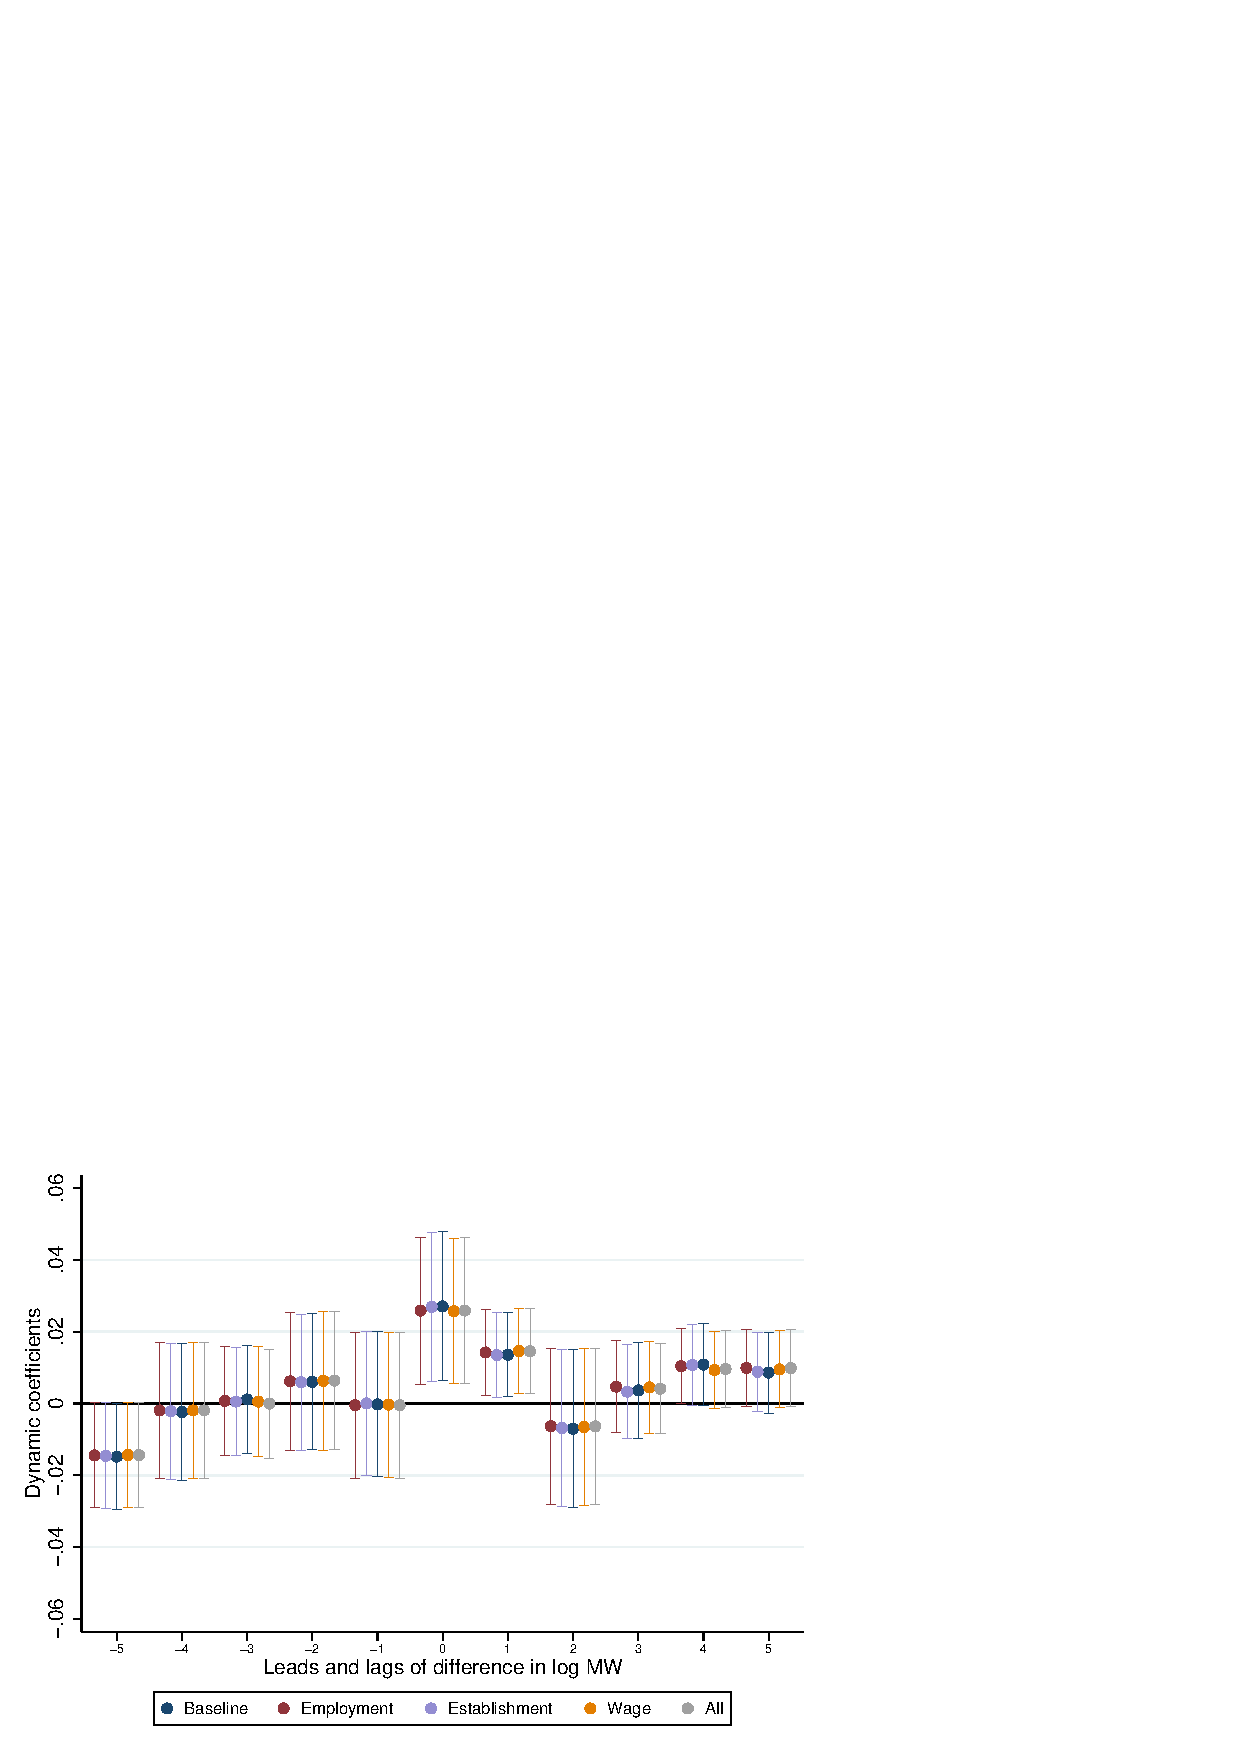
\includegraphics[width = 0.7\textwidth]{../../analysis/first_differences/output/fd_models_control.png}
    \begin{minipage}{.95\textwidth} \footnotesize
		\vspace{2mm} 
		\textit{Notes}: The figure show estimates for $\hat{\beta}_{r}$ obtained from 
		\autoref{eq:leads_lags} when progressively adding time-varying controls for local shocks. 
		The \textit{baseline} series plots coefficients taken from 
		\autoref{tab:dynamic_leads_lags_econshock}, column (1). The \textit{employment}, 
		\textit{establishment}, \textit{wage}, and \textit{building} series plot coefficients 
		from \autoref{tab:dynamic_leads_lags_econshock}, columns (2) to (5) respectively. 90 
		percent confidence intervals reported.  
	\end{minipage}
\end{figure}